\documentclass[]{beamer}
\usepackage[T1]{fontenc}
\usepackage[utf8]{inputenc}
\usepackage{lmodern}
\usepackage[italian]{babel}
\usepackage{mathrsfs}
\usepackage{cancel}

\title{Il potenziale elettrico}
\author{\texorpdfstring{Mattia Cozzi\newline\href{mailto:cozzimattia@gmail.com}{\texttt{cozzimattia@gmail.com}}}{Mattia Cozzi}}
\date{a.s.~2023/2024}

%\documentclass[handout]{beamer}     %usare questa classe per generare l'handout
%\usepackage{pgfpages}   %per mostrare più quadri nella stessa pagina
%\pgfpagesuselayout{4 on 1}[a4paper,border shrink=5mm,landscape]
\usetheme{Singapore}
%\useoutertheme[left]{sidebar} %elementi intorno alle diapositive
\setbeamercovered{dynamic} %modifica l'aspetto del testo grigetto delle diapositive future. Argomenti: invisible/transparent/dynamic
\usecolortheme{orchid}
% %COLORE PRINCIPALE
\definecolor{marroncino}{RGB}{156, 26, 0} % UBC Blue (primary)
\setbeamercolor{structure}{fg=marroncino} % itemize, enumerate, etc

\theoremstyle{plain}
\newtheorem{teorema}{Teorema}

\usepackage{tikz}
\usepackage{circuitikz}

\usepackage{pgf,pgfplots,graphicx}
\usetikzlibrary{angles,quotes,arrows,shapes,decorations.markings}
\pgfplotsset{compat=1.15}
\usepgfplotslibrary{units,fillbetween} % to add units easily to axis

\newcommand{\fem}{f_{em}}

\def\angolo[#1](#2)(#3:#4:#5)% Syntax: [draw options] (center) (initial angle:final angle:radius)
    { \draw[#1] ($(#2)+({#5*cos(#3)},{#5*sin(#3)})$) arc (#3:#4:#5); }


\begin{document}

\begin{frame}
  \titlepage
\end{frame}





\begin{frame}
\frametitle{Contenuti}
\tableofcontents
\end{frame}


\section{Energia potenziale}



\begin{frame}
\frametitle{Energia potenziale di due cariche (1)}
Immaginiamo un sistema di due cariche puntiformi, $ q_1 $ e $ q_2 $, poste a distanza $ r $.
\begin{figure}
\begin{tikzpicture}[scale=0.5]
\draw [] (6,0) -- (0,0);
\node [above,red] at (6,.3) {$ q_2 $};
\draw [red, ultra thick,fill=red] (6,0) circle [radius=.3];
\node [above] at (3,0) {$ r $};
\node [above,red] at (0,.3) {$ q_1 $};
\draw [red, ultra thick,fill=red] (0,0) circle [radius=.3];
\end{tikzpicture}
\end{figure}\pause
Definiamo l'energia potenziale elettrica del sistema come:
\begin{center}
\colorbox{marroncino!30}{$ U(r) = k_0 \dfrac{q_1 \, q_2}{r} $}
\end{center}
\end{frame}



\begin{frame}
\frametitle{Energia potenziale di due cariche (2)}
Nella definizione precedente, abbiamo assegnare il valore $ 0 $ dell'energia potenziale alla situazione in cui le due cariche sono a distanza infinita.
\pause

~

In effetti:
\begin{center}
$ \displaystyle \lim_{r \to + \infty} k_0 \dfrac{q_1 \, q_2}{r} = 0 $
\end{center}\pause

\begin{block}{Definizione di energia potenziale elettrica}
L'energia potenziale elettrica è il lavoro compiuto dalla forza di Coulomb quando le cariche sono portate a distanza infinita tra loro.
\end{block}
\end{frame}




\section{Potenziale}


\begin{frame}
\frametitle{Potenziale elettrico}
Definiamo il potenziale elettrico $ V_A $ del punto $ A $ come:
\begin{center}
\colorbox{marroncino!30}{$ V_A = \dfrac{U_A}{q_p} $}
\end{center}
Il potenziale elettrico si misura in \emph{volt}: $ 1 \, V = 1 \, \dfrac{J}{C} $.\pause
\end{frame}





\begin{frame}
\frametitle{Moto spontaneo delle cariche}
Se tra i punti $ A $ e $ B $ esiste una differenza di potenziale $ \Delta V $ per cui \alert{$ V_A > V_B $} (cioè il punto $ A $ è ad alto potenziale e $ B $ è a basso potenziale), avremo i seguenti moti spontanei:
\begin{figure}
\begin{tikzpicture}[scale=0.5]
\draw [->,thick,gray] (3,0) -- (5,0);
\draw [->,thick,gray] (0,0) -- (-2,0);
\draw [|-|,thick] (-6,-2) -- (9,-2);
\node [below] at (1.5,-2.3) {$ \Delta V $};
\node [above,red] at (3,.2) {$ q_+ $};
\node [below] at (-6,0) {$ A $};
\node [below] at (9,0) {$ B $};
\draw [ultra thick,fill] (-6,0) circle [radius=.1];
\draw [ultra thick,fill] (9,0) circle [radius=.1];
\draw [red, ultra thick,fill=red] (3,0) circle [radius=.2];
\node [above,blue] at (0,.2) {$ q_- $};
\draw [blue, ultra thick,fill=blue] (0,0) circle [radius=.2];
\end{tikzpicture}
\end{figure}\pause
La differenza di potenziale è detta anche \alert{tensione}.
\end{frame}


\section{Superfici}

\begin{frame}
\frametitle{Superfici equipotenziali}
Analogamente a quanto fatto con le linee del campo elettrico, possiamo trovare un modo per visualizzare il potenziale elettrico.

\begin{block}{Superficie (linea) equipotenziale}
Una superficie (linea) equipotenziale è l'insieme dei punti dello spazio in cui il potenziale elettrico assume il medesimo valore.
\end{block}
\end{frame}




\begin{frame}
\frametitle{Superfici equipotenziali e linee del campo}
\begin{columns}
\begin{column}{0.25\textwidth}
\begin{figure}
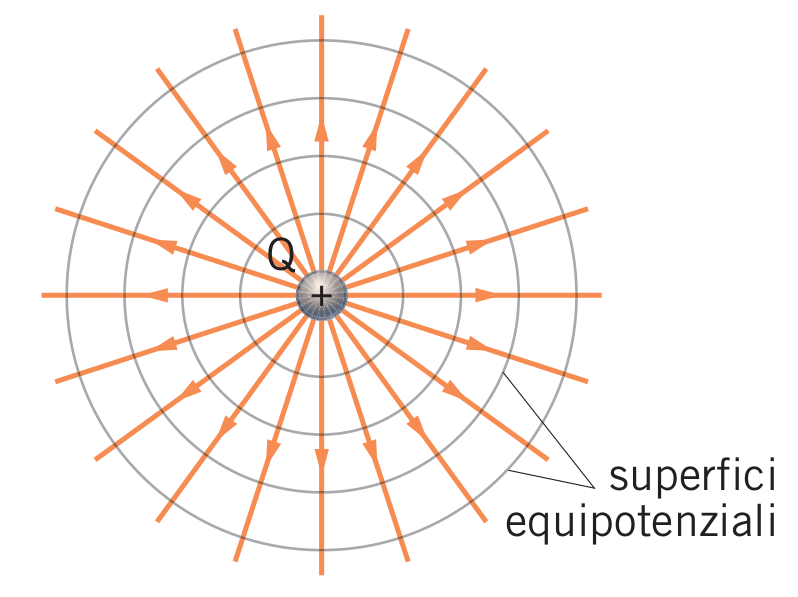
\includegraphics[width=\columnwidth]{img/superficieequipotenziale1.png}
\end{figure}
\end{column}
\begin{column}{0.25\textwidth}
\begin{figure}
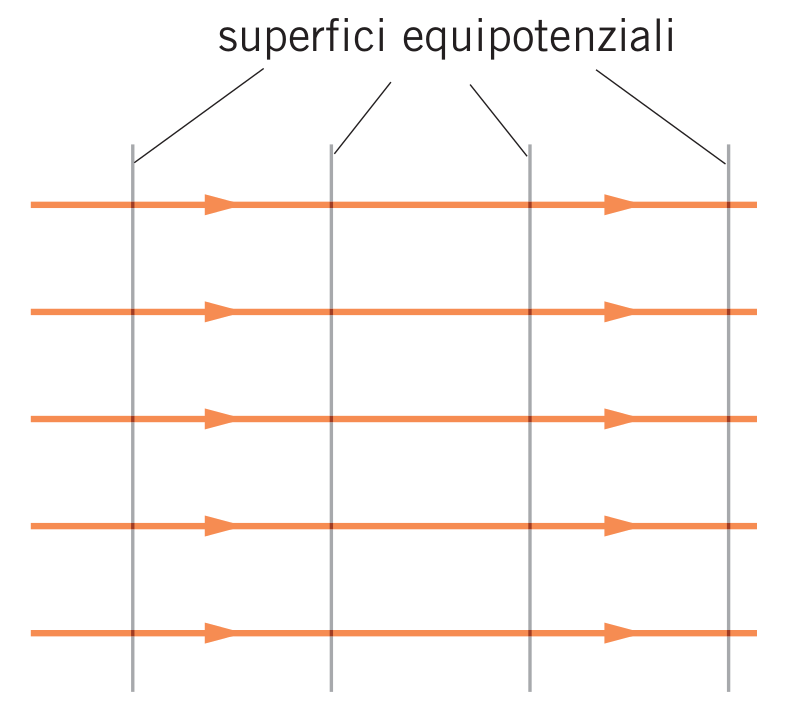
\includegraphics[width=\columnwidth]{img/superficieequipotenziale2.png}
\end{figure}
\end{column}
\begin{column}{0.5\textwidth}
\begin{figure}
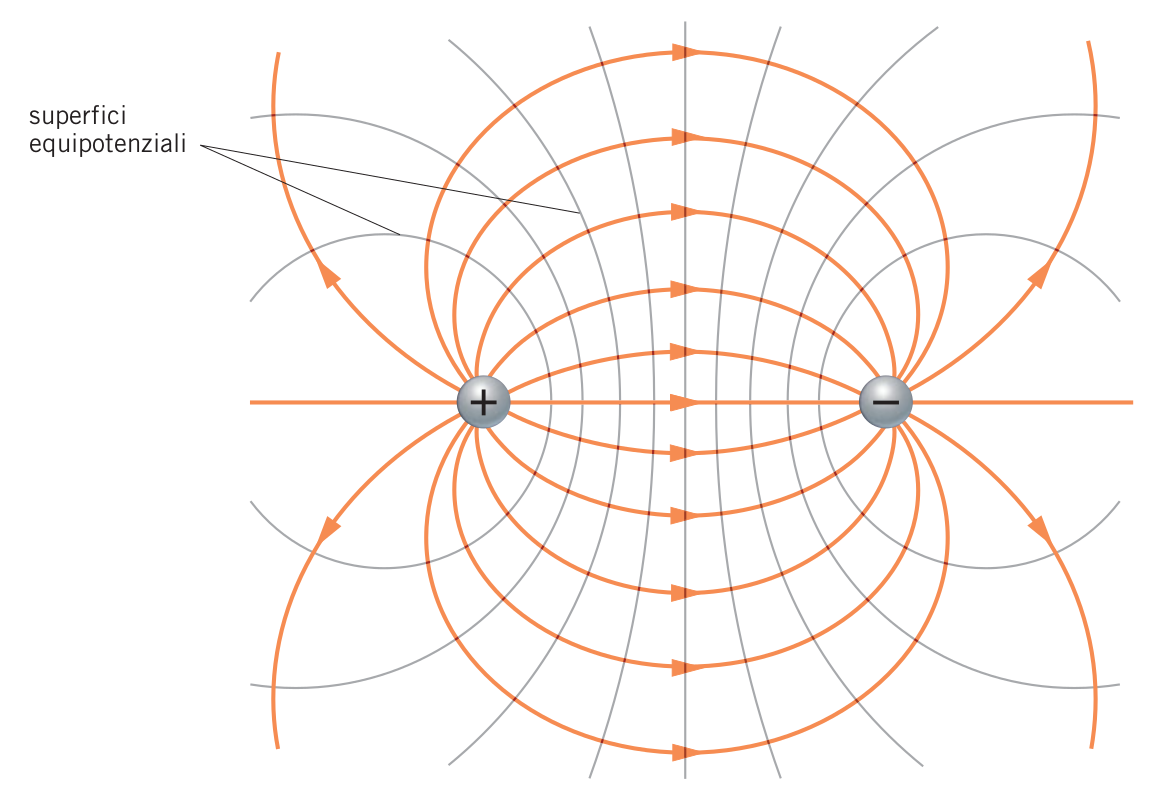
\includegraphics[width=\columnwidth]{img/superficieequipotenziale3.png}
\end{figure}
\end{column}
\end{columns}\pause

~

\alert{Le linee del campo elettrico sono sempre perpendicolari alle superfici (linee) equipotenziali.}
\end{frame}


\end{document}
